\section{Software Development and Lifecycle}

A large scale software system involves many interconnected components, all of which must adhere to essential software development principles. The goal is not just to write code but to build a system that is reliable, maintainable, scalable, and efficient. Ensuring the system is free of bugs and capable of adapting to future needs is as important as the initial development itself. By following these key paradigms, developers can create software that meets high standards of quality and performance.

\begin{figure}[H]
    \centering
    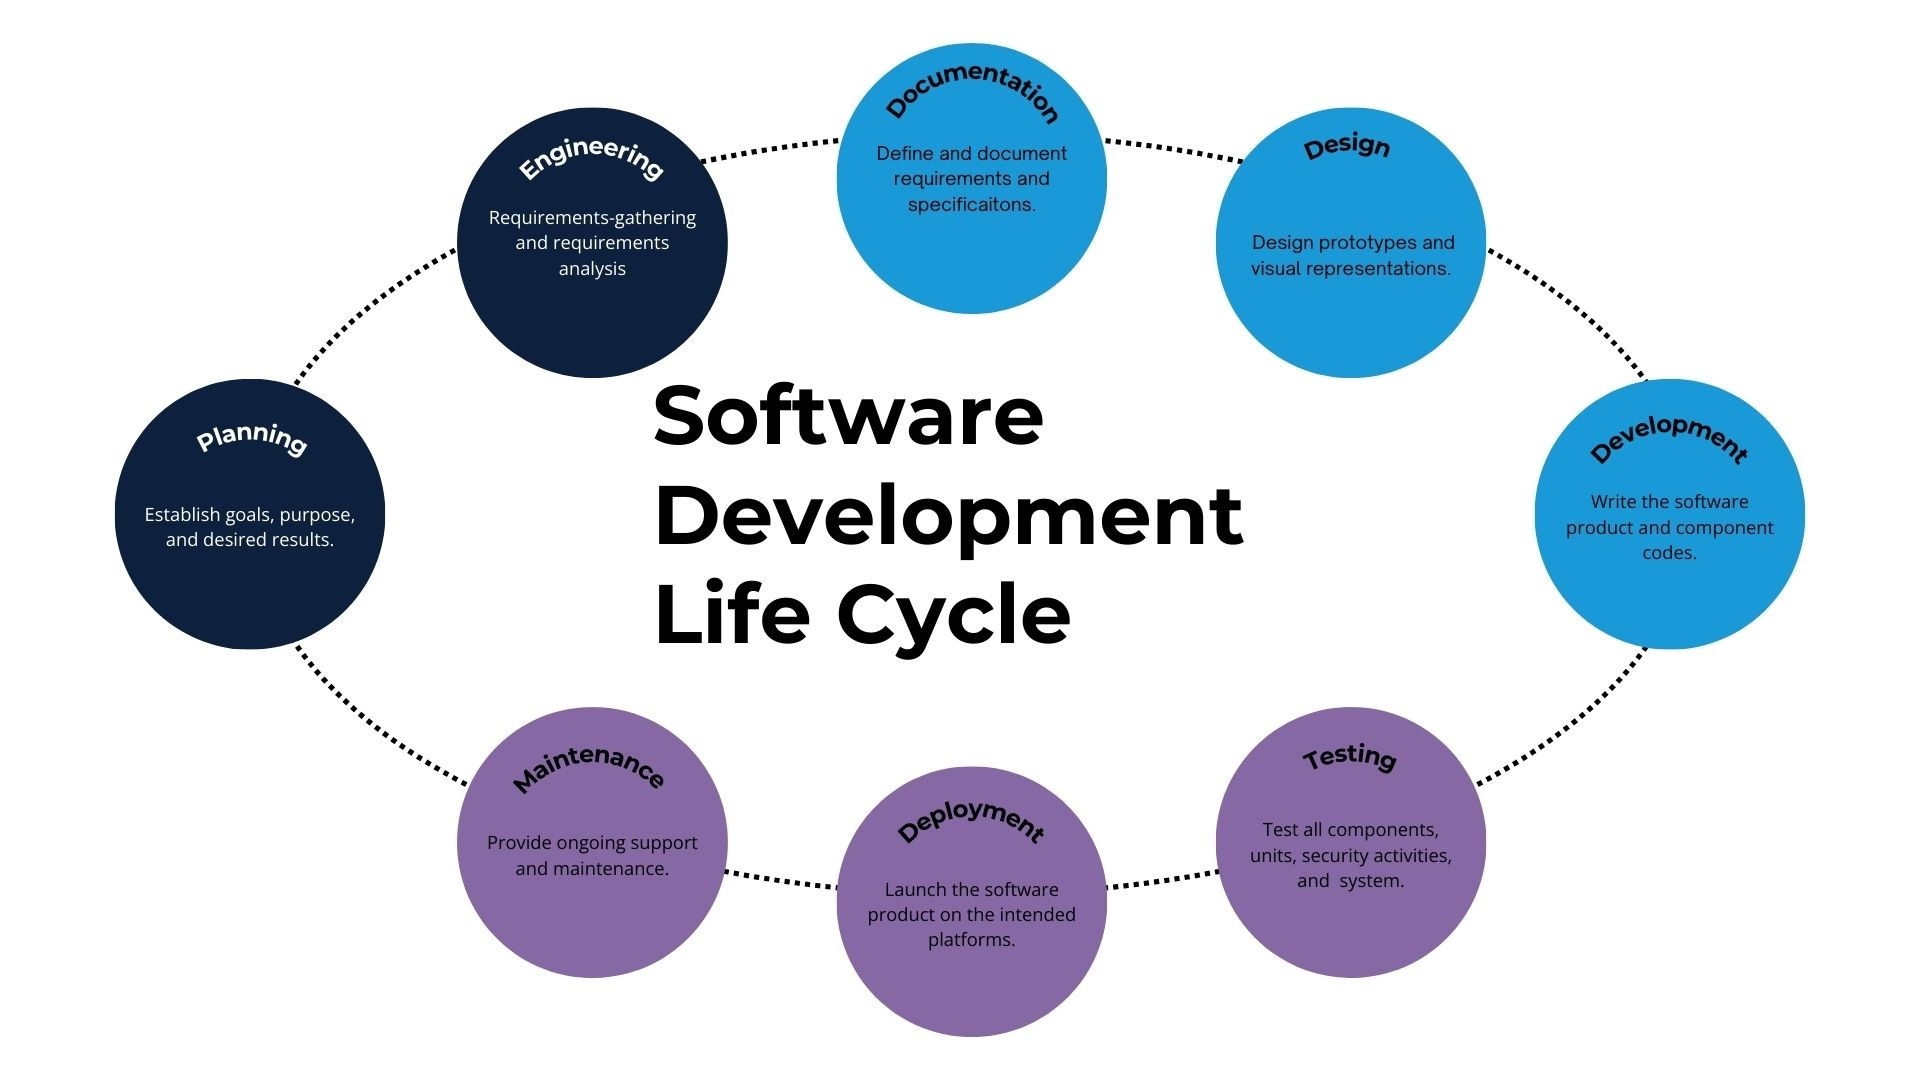
\includegraphics[width=0.8\textwidth]{figures/software_development.png}
    \caption[Software Development Life cycle]{Software Development Life cycle\par (adapted from~\cite{sire_sdlc_2024})}
	\label{fig:background_sd}
\end{figure}

\autoref{fig:background_sd} illustrates the software development life cycle. Each phase of the software development lifecycle process adds an important contribution to the overall project. For example, in the planning and engineering phase, the team works closely with stakeholders to determine the functional and non-functional requirements of the project. This collaboration ensures that everyone involved understands the project's goals and technical needs. In the documentation phase, all the information gathered during planning and engineering is carefully recorded. This creates a detailed reference for the team, helping maintain consistency and clarity as the project progresses.

Following the \textit{Software Development Life Cycle (SDLC)} provides several key benefits. It helps in identifying clear goals, ensures all stakeholders are on the same page, and allows for thorough testing at every stage. This structured approach produces high-quality software systems and maintains a smooth and understandable development flow. By sticking to the \textit{SDLC}, teams can reduce risks, avoid confusion, and create software that meets user expectations.

Once the major development work is complete, the focus shifts to software maintenance. Maintaining a large project becomes a significant task in itself. Updates, bug fixes, and adapting to new requirements or technologies are ongoing responsibilities. Without proper maintenance, even the best-designed systems can become outdated or difficult to use.

Another challenge that arises is understanding the system once it has been completed. Software development often requires years of effort and large amount of resources. As a result, understanding the full complexity of a system after its development can be difficult, especially for teams that were not part of the original project. Proper documentation, clear workflows, and thorough knowledge transfer are critical to addressing this issue. However, even with these measures, there are instances where critical system insights are required to understand the system. This is why reverse engineering is often applied to existing or legacy systems to gain a clear understanding of their structure and functionality.